\documentclass[a4paper,11pt]{article}
\usepackage[T1]{fontenc}
\usepackage[utf8]{inputenc}
\usepackage[francais]{babel}
\usepackage{lmodern}
\usepackage{hyperref}
\usepackage{graphicx}

\title{{\sc Warlogo}\\{\small Prise en main d'un jeu de guerre dont vous êtes le héros en NetLogo}}
\author{Jacques Ferber \and Fabien Hervouet \and Loïs Vanhée}
\date{FMIN207 -- M1 Informatique\\TP Programmation Orientée Agents \\
Nov. 2019}

\begin{document}

\maketitle


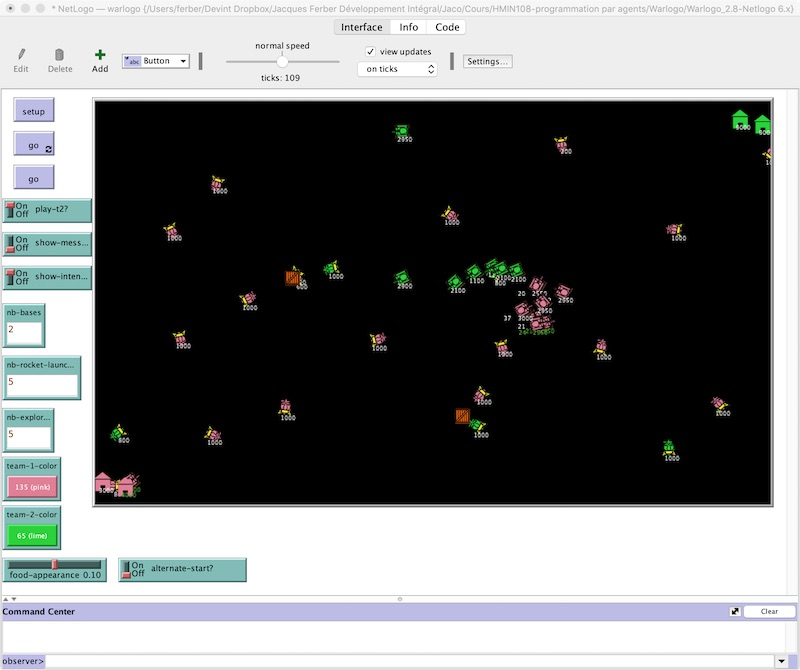
\includegraphics{warlogo.jpg}

%%%%%%%%%%%%%%%%%%%%%%%%%%%%%%%%%%%%%%%%%%%%%%%%%%%%%%%%%%%%
\section*{Introduction}


%%%%%%%%%%%%%%%%%%%%%%%%%%%%%%
\subsection*{Warlogo}

\texttt{Warlogo} est la réécriture en \textit{NetLogo} de la plateforme \texttt{Warbot}, dédiée à la
simulation dans un environnement logique et graphique d'un jeu de stratégie pour y intégrer une
intelligence artificielle agissant au niveau individuel. Divers projets similaires existent pour des
jeux du marché (par exemple \textit{Pogamut} permet d'intégrer des agents  pour \textit{Unreal
Tournament} et \textit{Defcon}). L'outil développé ici est volontairement plus simple pour vous
permettre de produire une IA simple rapidement tout en laissant la possibilité à ceux qui le
souhaitent de complexifier le comportement de leurs agents.\\

L'objectif de ce TP est de développer des agents au comportement intelligent afin de satisfaire le
but du jeu : détruire la base ennemie à l'aide de ses robots. La définition d'agent est encore floue
dans la communauté mais en voici une idée simple. Un agent est un ``esprit'' qui habite un
``corps''.  Cet ``esprit'' ne peut voir qu'au travers des yeux de son ``corps'' et ne peut agir que
via les effecteurs de son corps (bras, jambes). Plus formellement, votre agent a le pouvoir de
\textbf{percevoir} via son environnement et doit \textbf{décider d'une action} à réaliser.
L'environnement décidera du résultat de son action (et celle des autres agents) et lui fournira de
nouveaux percepts.\\

Dans ce document, vous trouverez tout ce dont vous avez besoin pour connaitre le fonctionnement de
l'environnement, des percepts et des actions.

%%%%%%%%%%%%%%%%%%%%%%%%%%%%%%
\subsection*{Les différents types d'agents}

Il y a trois types de corps dont vous aurez à programmer le comportement : \texttt{bases},
\texttt{explorers}, \texttt{rocket-launchers}.

%%%%%%%%%%%%%%%
\subsubsection*{Bases}
Les \texttt{bases} représentent le quartier général de votre équipe. Ce sont des agents ne pouvant
pas se déplacer physiquement dans le monde. En revanche elles peuvent construire des unités de type
\texttt{explorers} et \texttt{rocket-launchers}.

%%%%%%%%%%%%%%%
\subsubsection*{Explorers}
Les \texttt{explorers} sont des agents dédiés à l'exploration du monde. Ils sont pacifistes et ne
peuvent donc pas attaquer d'unités ennemies. Ils peuvent se déplacer et servent donc essentiellement
à découvrir le territoire, le surveiller, récupérer de l'énergie sous forme de nourriture dispersée
dans l'environnement. À terme ils permettront de donner des informations sur le reste du monde aux
autres agents grâce à un module de communication.

%%%%%%%%%%%%%%%
\subsubsection*{Rocket-launchers}
Les \texttt{rocket-launchers} sont les seules unités à pouvoir se battre. Ils peuvent se déplacer
dans l'environnement et tirer des missiles (qui affectent les amis comme les ennemis). Ils ne
peuvent tirer un missile que tout les $k$ tours ($k$ étant par défaut défini à 3). Ils disposent
d'un certain nombre de missiles. Quand ils n'ont plus de missiles, ils ne peuvent plus tirer.
Cependant, ils ont la possibilité de perdre de la vie pour construire un missile.



%%%%%%%%%%%%%%%%%%%%%%%%%%%%%%%%%%%%%%%%%%%%%%%%%%%%%%%%%%%%
\section*{Fonctionnement global du programme}

Le paradigme agent limite vos possibilités de perception et d'action sur l'environnement à
l'\texttt{API} que nous vous proposons. Imaginez-vous enfermé dans un sous-marin. Vous avez pour
seule information un moniteur qui vous délivre certaines informations (écho sonar, état de la
coque...) et un ensemble de manettes à tirer devant vous. La carelingue et l'océan décident pour
vous du résultat. Essayez de vous placer en vue subjective.\\

Les contraintes techniques de NetLogo vous permettent de prendre le contrôle de l'océan (et du reste
de l'univers) ! Ignorez-les, en pratique vous ne les avez pas. Par conséquent il est
\textbf{interdit} de modifier n'importe quelle variable autre que sa tâche, ses croyances et les
variables locales. Il est aussi interdit de lire des informations que l'agent ne possède pas dans
ses percepts ou dans ses messages.\\

Pour finir, il est interdit de garder un pointeur sur un agent en mémoire. En revanche, vous avez le
droit de garder toutes les informations d'un agent perçu (son numéro, son énergie...). La raison est
que (pour des raisons de simplicité et d'efficacité), nous vous fournissons en perception des
pointeurs sur les autres agents. Si vous mémorisez ce pointeur et que l'agent sort de votre champ
perceptif... vous avez toujours accès aux informations (mises à jour) de cet agent, alors que vous
devriez, au mieux, ne pouvoir vous souvenir que des informations de votre dernière rencontre.

%%%%%%%%%%%%%%%%%%%%%%%%%%%%%%
\subsection*{Les actions}

Chaque action coûte un tour à l'agent. Vous devez donc soigneusement choisir la meilleure action à lui
faire effectuer en fonction du contexte qu'il perçoit de son environnement.

\begin{description}
  \item[\texttt{move}] Permet à n'importe quel agent de se déplacer dans l'environnement sachant
    qu'il peut se retrouver bloqué (contre un mur par exemple).
  \item[\texttt{take [o]}] Permet à un robot de prendre la ressource \texttt{o} dans
    l'environnement et de la placer dans son sac. Si le sac est plein, rien ne de passe.
  \item[\texttt{eat}] Permet à n'importe quel agent de manger de la nourriture emmagasinée dans son
    sac pour regagner de l'énergie.
  \item[\texttt{give [a]}] Permet à n'importe quel agent de donner de la nourriture contenue dans
    son sac à l'agent \texttt{a}, à condition qu'il soit suffisamment proche.
  \item[\texttt{drop}] Permet à un agent de se délester d'une unité de nourriture contenue dans son
    sac.
  \item[\texttt{put-smell [s]}] Permet à un agent de déposer \texttt{s} de phéromones sur le patch
    courant.
  \item[\texttt{idle}] État d'oisiveté.
  \item[\texttt{build-rocket}] Permet à un agent de type \texttt{rocket-launcher} de construire un
    missile.
  \item[\texttt{launch-rocket [t]}] Permet à un agent de type \texttt{rocket-launcher} d'envoyer un
    missile déjà construit dans la direction \texttt{t} (valeur de l'angle).
  \item[\texttt{build-explorer}] Permet à un agent de type \texttt{base} de créer un agent de type
    \texttt{explorer}.
  \item[\texttt{build-rocket-launcher}] Permet à un agent de type \texttt{base} de créer un agent de
    type \texttt{rocket-launcher}.\\
\end{description}

Les actions suivantes en revanche ne coûtent rien et redéfinissent l'\texttt{API} par défaut de
NetLogo.

\begin{description}
  \item[\texttt{set-heading [a]}] Permet de changer la direction de n'importe quel agent (\texttt{a}
    pouvant être un agent ou un nombre représentant l'angle).
  \item[\texttt{set-random-heading}] Permet de changer aléatoirement la direction de n'importe quel
    agent.
\end{description}

%%%%%%%%%%%%%%%%%%%%%%%%%%%%%%
\subsection*{Les primitives de tests}

Des primitives de tests ont été mises en place pour vous faciliter le travail. Elles renvoient des
valeurs booléennes sur des choses que vous aurez très souvent à évaluer avant d'agir.

\begin{description}
  \item[\texttt{is-base? [a]}] Renvoie \texttt{vrai} si l'unité est de type \texttt{base}, \texttt{faux} sinon.
  \item[\texttt{is-explorer? [a]}] Renvoie \texttt{vrai} si l'unité est de type \texttt{explorer}, \texttt{faux} sinon.
  \item[\texttt{is-rocket-launcher? [a]}] Renvoie \texttt{vrai} si l'unité est de type \texttt{rocket-launcher}, \texttt{faux} sinon.
  \item[\texttt{is-robot? [a]}] Renvoie \texttt{vrai} si l'unité à qui vous demandez cela est soit de
    type \texttt{base}, \texttt{explorer} ou \texttt{rocket-launcher}, \texttt{faux} sinon.
  \item[\texttt{is-food? [a]}] Renvoie \texttt{vrai} si l'unité est de type \texttt{food}, \texttt{faux} sinon.
  \item[\texttt{is-rocket? [a]}] Renvoie \texttt{vrai} si l'unité est de type \texttt{rocket}, \texttt{faux} sinon.
  \item[\texttt{is-my-friend? [a]}] Renvoie \texttt{vrai} si $a$ cela appartient à
    votre équipe, \texttt{faux} sinon.
  \item[\texttt{is-my-enemy? [a]}] Renvoie \texttt{faux} si $a$ appartient à
    votre équipe, \texttt{vrai} sinon.
 \item[\texttt{are-enemies? [$a_1$ $a_2$]}] Renvoie \texttt{vrai} si $a_1$ et $a_2$ sont ennemis,  \texttt{faux}  sinon.
\item[\texttt{are-friends? [$a_1$ $a_2$]}] Renvoie \texttt{vrai} si $a_1$ et $a_2$ sont amis,  \texttt{faux}  sinon.
  \item[\texttt{is-colliding? [a]}] Renvoie \texttt{vrai} si l'agent appelant est en collision avec l'agent
    \texttt{a}, \texttt{faux} sinon.
  \item[\texttt{headed-towards? [a]}] Renvoie \texttt{vrai} si l'agent est déjà dans la direction de
    l'agent \texttt{a}, \texttt{faux} sinon.
  \item[\texttt{in-base?}] Renvoie vrai si l'agent se situe dans une \texttt{base} amie.
  \item[\texttt{blocked?}] Renvoie \texttt{vrai} si l'agent est bloqué quelquepart dans
    l'environnement, \texttt{faux} sinon.
  \item[\texttt{empty-bag?}] Renvoie \texttt{faux} si il reste de la nourriture dans le sac,
    \texttt{vrai} sinon.
  \item[\texttt{full-bag?}] Renvoie \texttt{vrai} si le sac de l'agent est plein, \texttt{faux}
    sinon.
  \item[\texttt{hitting-north-wall? [a]}] Renvoie \texttt{vrai} si $a$ percute le mur Nord, \texttt{faux}
    sinon.
  \item[\texttt{hitting-south-wall? [a]}] Renvoie \texttt{vrai} si $a$ percute le mur Sud, \texttt{faux}
    sinon.
  \item[\texttt{hitting-east-wall? [a]}] Renvoie \texttt{vrai} si $a$ percute le mur Est, \texttt{faux}
    sinon.
  \item[\texttt{hitting-west-wall? [a]}] Renvoie \texttt{vrai} si $a$ percute le mur Ouest, \texttt{faux}
    sinon.

\end{description}

%%%%%%%%%%%%%%%%%%%%%%%%%%%%%%
\subsection*{Les primitives de perception}

Des primitives de perception ont été mises en place pour vous faciliter le travail. Elles renvoient
des valeurs sur des choses que vous aurez très souvent à évaluer avant d'agir.

\begin{description}
  \item[\texttt{get-team}] Renvoie la couleur de l'équipe à laquelle l'agent appartient.
  \item[\texttt{get-energy [a]}] Renvoie le taux d'énergie de l'agent $a$.
  \item[\texttt{percepts}] Renvoie la liste de tous les percepts/agents détectés par l'agent.
  \item[\texttt{get-bases}] Renvoie l'agentset des \texttt{bases} amies.
  \item[\texttt{get-rocket-launchers}] Renvoie l'agentset des \texttt{rocket-launchers} amis.
  \item[\texttt{get-explorers}] Renvoie la liste des \texttt{explorers} amies.
  \item[\texttt{get-heading}] Renvoie l'angle d'orientation de l'agent.
  \item[\texttt{get-rocket-number}] Renvoie le nombre de missiles restant à l'agent.
  \item[\texttt{carriable-lenght}] Renvoie la taille du sac de l'agent, correspondant au nombre
    d'objets qu'il peut conserver avec lui.
  \item[\texttt{smell-friend}] Renvoie la valeur du phéromone propre à l'équipe amie sur le patch
    courant.
  \item[\texttt{smell-enemy}] Renvoie la valeur du phéromone propre à l'équipe ennemie sur le patch
    courant.
\end{description}

%%%%%%%%%%%%%%%%%%%%%%%%%%%%%%
\subsection*{Communication entre agents}

Un module permettant de faire communiquer les agents entre eux a été mis en place. Ce module est
censé vous permettre d'améliorer la couche cognitive de vos agents et de leur permettre de coopérer
plus finement.\\

Pour pouvoir envoyer des messages à d'autres agents, deux primitives sont à disposition :
\texttt{send-message [receiver performative content]} et \texttt{broadcast-message [receivers
performative content]}. La première permet d'envoyer un message à un seul agent, alors que la
seconde permet d'envoyer le même message à tous les agents d'un \texttt{agentset} passé en
paramètre. Voici un exemple de leur utilisation :

\begin{verbatim}
  let enemy-base one-of percepts with [is-base? self and is-my-enemy? myself]
  let my-base one-of get-bases
  if enemy-base != nobody and my-base != nobody [
    send-message my-base "seen-base" [] 
    broadcast-message get-rocket-launchers "attack" [] 
  ]
\end{verbatim}

Chaque agent dispose d'un attribut \texttt{incoming-queue}, dans lequel sont stockés les messages
reçus. Les messages sont caractérisés par un expéditeur (\texttt{get-sender [msg]}), un performatif
(\texttt{get-performative [msg]}), un contenu (\texttt{get-content [msg]}), la direction de
l'expéditeur par rapport au receveur (\texttt{get-heading-to-sender [msg]}) et la distance qui
sépare l'expéditeur du receveur (\texttt{get-distance-to-sender [msg]}). Une troisième primitive
d'envoi de message est disponible pour permettre de répondre très facilement à un message reçu :
\texttt{reply [msg performative content]}. Pour pouvoir agir en fonction de ces messages, dans la
boucle de vie de votre agent, il est recommandé d'utiliser la structure suivante :

\begin{verbatim}
  while [not empty? incoming-queue] [
    let msg get-message
    show get-sender msg
    show get-performative msg
    show get-content msg
    show get-heading-to-sender msg
    show get-distance-to-sender msg
    reply msg "ack" []
  ]
\end{verbatim}

%%%%%%%%%%%%%%%%%%%%%%%%%%%%%%
\subsection*{Définition de comportement}

Un comportement de base est fourni pour chacun des trois types d'agents ennemis. Cela va vous
permettre de pouvoir vous mesurer localement à des agents basiques avant de pouvoir vous mettre en
situation de compétition avec les autres étudiants. Vous devez donc vous occuper uniquement de la
programmation des cerveaux de vos agents. Pour définir par vous-même un comportement pour chacun des
trois types d'agents, vous allez devoir changer les trois méthodes suivantes :

\begin{verbatim}
  to-report base-t1-action
    ...
  end
  
  to-report explorer-t1-action
    ...
  end
  
  to-report rocket-launcher-t1-action
    ...
  end
\end{verbatim}

Ces trois fonctions doivent toujours soit retourner une simple chaîne de caractère (\texttt{report
"move"}), soit une liste (\texttt{report list "take" object}), correspondant à l'action à faire
exécuter à l'agent.\\

En pratique, vous devez télécharger l'archive qui se trouve sur le site
\href{http://www.warbot.fr}{www.warbot.fr} comprenant quatre fichiers : \texttt{warlogo.nlogo},
\texttt{warlogo-core.nls}, \texttt{warlogo-communication.nls} et \texttt{warlogo-basicIA.nls}. Vous
devez extraire ces fichiers dans un même dossier. Puis il vous suffit de lancer \texttt{NetLogo} et
d'ouvrir le fichier \texttt{warlogo.nlogo}. C'est dans ce fichier que vous allez programmer le
comportement de vos agents.

\end{document}
